\documentclass{standalone}
\usepackage{tikz}
\usetikzlibrary{patterns, positioning}

\begin{document}
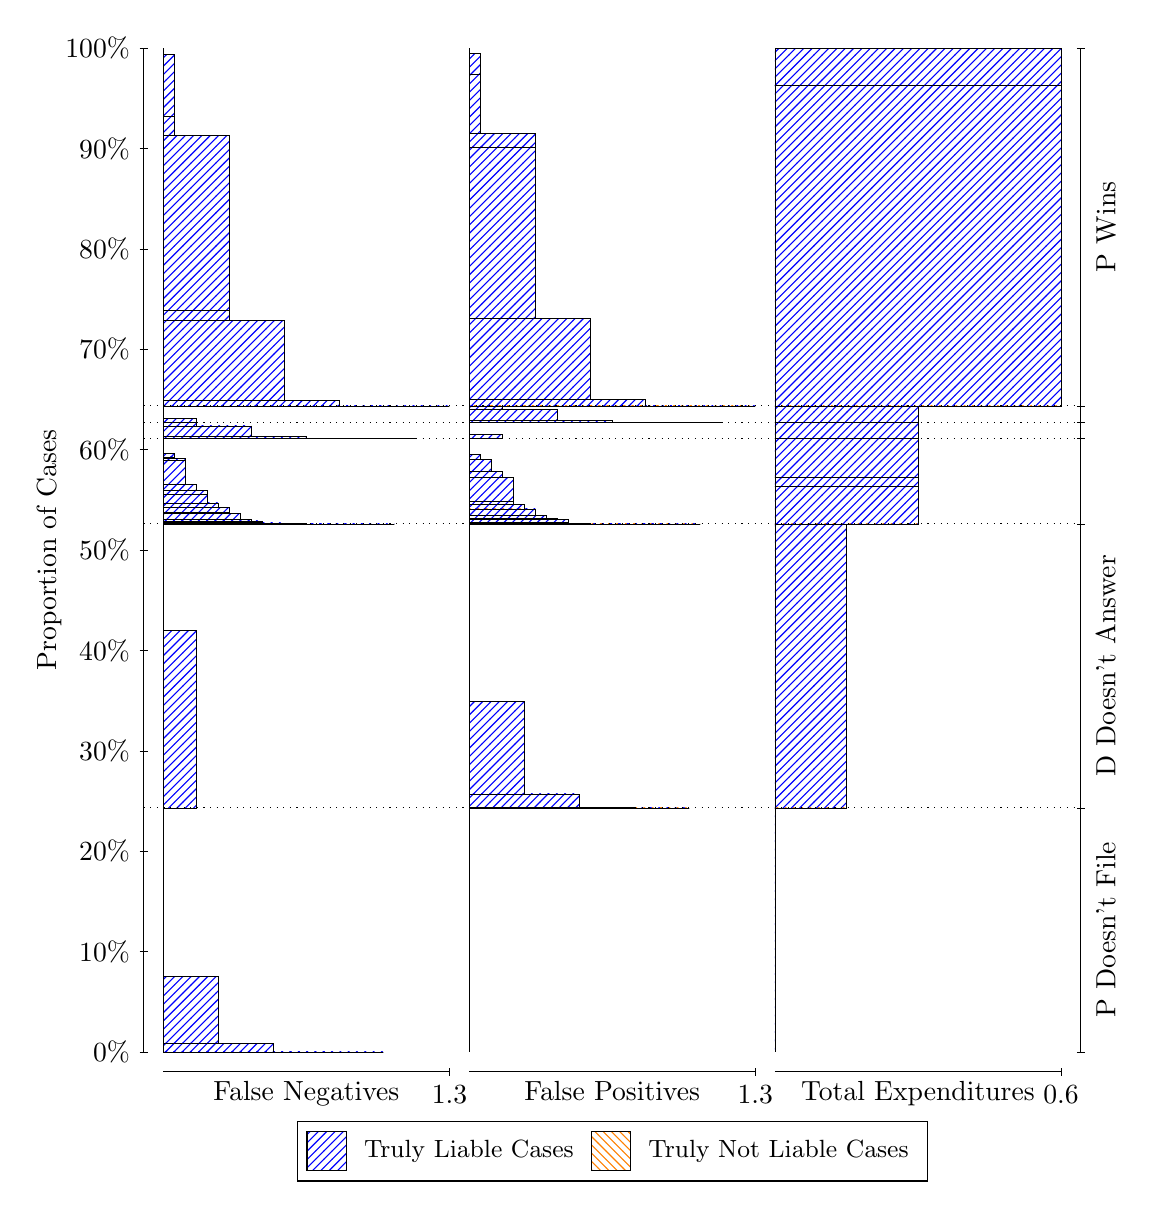
\begin{tikzpicture}
\draw[black, very thin] (1.5,1.75) -- (1.5,14.5);
\node[rotate=90, anchor=center] at (0.3, 8.125) {Proportion of Cases};
\draw[black, very thin] (1.45,1.75) -- (1.55,1.75);
\node[anchor=east] at (1.45, 1.75) {0\%};
\draw[black, very thin] (1.45,3.025) -- (1.55,3.025);
\node[anchor=east] at (1.45, 3.025) {10\%};
\draw[black, very thin] (1.45,4.3) -- (1.55,4.3);
\node[anchor=east] at (1.45, 4.3) {20\%};
\draw[black, very thin] (1.45,5.575) -- (1.55,5.575);
\node[anchor=east] at (1.45, 5.575) {30\%};
\draw[black, very thin] (1.45,6.85) -- (1.55,6.85);
\node[anchor=east] at (1.45, 6.85) {40\%};
\draw[black, very thin] (1.45,8.125) -- (1.55,8.125);
\node[anchor=east] at (1.45, 8.125) {50\%};
\draw[black, very thin] (1.45,9.4) -- (1.55,9.4);
\node[anchor=east] at (1.45, 9.4) {60\%};
\draw[black, very thin] (1.45,10.675) -- (1.55,10.675);
\node[anchor=east] at (1.45, 10.675) {70\%};
\draw[black, very thin] (1.45,11.95) -- (1.55,11.95);
\node[anchor=east] at (1.45, 11.95) {80\%};
\draw[black, very thin] (1.45,13.225) -- (1.55,13.225);
\node[anchor=east] at (1.45, 13.225) {90\%};
\draw[black, very thin] (1.45,14.5) -- (1.55,14.5);
\node[anchor=east] at (1.45, 14.5) {100\%};

\draw[black, very thin] (13.4,1.75) -- (13.4,14.5);
\draw[black, very thin] (13.35,1.75) -- (13.45,1.75);
\node[anchor=west] at (13.35, 1.75) {};
\draw[black, very thin] (13.35,4.851) -- (13.45,4.851);
\node[anchor=west] at (13.35, 4.851) {};
\draw[black, very thin] (13.35,8.4574) -- (13.45,8.4574);
\node[anchor=west] at (13.35, 8.4574) {};
\draw[black, very thin] (13.35,9.5435) -- (13.45,9.5435);
\node[anchor=west] at (13.35, 9.5435) {};
\draw[black, very thin] (13.35,9.7491) -- (13.45,9.7491);
\node[anchor=west] at (13.35, 9.7491) {};
\draw[black, very thin] (13.35,9.9559) -- (13.45,9.9559);
\node[anchor=west] at (13.35, 9.9559) {};
\draw[black, very thin] (13.35,14.5) -- (13.45,14.5);
\node[anchor=west] at (13.35, 14.5) {};

\draw[black, very thin, pattern color=blue, pattern=north east lines] (1.75,1.75) rectangle (4.5449,1.75);
\draw[black, very thin, pattern color=blue, pattern=north east lines] (1.75,1.75) rectangle (3.8462,1.7509);
\draw[black, very thin, pattern color=blue, pattern=north east lines] (1.75,1.7509) rectangle (3.1474,1.8594);
\draw[black, very thin, pattern color=blue, pattern=north east lines] (1.75,1.8594) rectangle (2.4487,2.7078);
\draw[black, very thin, pattern color=orange, pattern=north west lines] (1.75,2.7078) rectangle (1.75,2.7078);
\draw[black, very thin, pattern color=blue, pattern=north east lines] (1.75,2.7078) rectangle (1.75,4.851);
\draw[black, very thin, pattern color=blue, pattern=north east lines] (1.75,4.851) rectangle (2.1692,7.1034);
\draw[black, very thin, pattern color=orange, pattern=north west lines] (1.75,7.1034) rectangle (1.75,7.1034);
\draw[black, very thin, pattern color=blue, pattern=north east lines] (1.75,7.1034) rectangle (1.75,8.4574);
\draw[black, very thin, pattern color=blue, pattern=north east lines] (1.75,8.4574) rectangle (4.6846,8.4574);
\draw[black, very thin, pattern color=blue, pattern=north east lines] (1.75,8.4574) rectangle (4.4051,8.4574);
\draw[black, very thin, pattern color=blue, pattern=north east lines] (1.75,8.4574) rectangle (4.1256,8.4574);
\draw[black, very thin, pattern color=blue, pattern=north east lines] (1.75,8.4574) rectangle (3.9859,8.4574);
\draw[black, very thin, pattern color=blue, pattern=north east lines] (1.75,8.4574) rectangle (3.8462,8.4574);
\draw[black, very thin, pattern color=blue, pattern=north east lines] (1.75,8.4574) rectangle (3.7064,8.4574);
\draw[black, very thin, pattern color=blue, pattern=north east lines] (1.75,8.4574) rectangle (3.5667,8.4592);
\draw[black, very thin, pattern color=blue, pattern=north east lines] (1.75,8.4592) rectangle (3.4269,8.4593);
\draw[black, very thin, pattern color=blue, pattern=north east lines] (1.75,8.4593) rectangle (3.2872,8.4687);
\draw[black, very thin, pattern color=blue, pattern=north east lines] (1.75,8.4687) rectangle (3.1474,8.4689);
\draw[black, very thin, pattern color=blue, pattern=north east lines] (1.75,8.4689) rectangle (3.0077,8.4831);
\draw[black, very thin, pattern color=blue, pattern=north east lines] (1.75,8.4831) rectangle (3.0077,8.4938);
\draw[black, very thin, pattern color=blue, pattern=north east lines] (1.75,8.4938) rectangle (2.8679,8.51);
\draw[black, very thin, pattern color=blue, pattern=north east lines] (1.75,8.51) rectangle (2.7282,8.5887);
\draw[black, very thin, pattern color=blue, pattern=north east lines] (1.75,8.5887) rectangle (2.5885,8.6027);
\draw[black, very thin, pattern color=blue, pattern=north east lines] (1.75,8.6027) rectangle (2.5885,8.6619);
\draw[black, very thin, pattern color=blue, pattern=north east lines] (1.75,8.6619) rectangle (2.4487,8.7228);
\draw[black, very thin, pattern color=blue, pattern=north east lines] (1.75,8.7228) rectangle (2.309,8.8295);
\draw[black, very thin, pattern color=blue, pattern=north east lines] (1.75,8.8295) rectangle (2.309,8.8797);
\draw[black, very thin, pattern color=blue, pattern=north east lines] (1.75,8.8797) rectangle (2.1692,8.9541);
\draw[black, very thin, pattern color=blue, pattern=north east lines] (1.75,8.9541) rectangle (2.0295,9.2634);
\draw[black, very thin, pattern color=blue, pattern=north east lines] (1.75,9.2634) rectangle (2.0295,9.2923);
\draw[black, very thin, pattern color=blue, pattern=north east lines] (1.75,9.2923) rectangle (1.8897,9.3083);
\draw[black, very thin, pattern color=blue, pattern=north east lines] (1.75,9.3083) rectangle (1.8897,9.355);
\draw[black, very thin, pattern color=blue, pattern=north east lines] (1.75,9.355) rectangle (1.75,9.3551);
\draw[black, very thin, pattern color=orange, pattern=north west lines] (1.75,9.3551) rectangle (1.75,9.3551);
\draw[black, very thin, pattern color=blue, pattern=north east lines] (1.75,9.3551) rectangle (1.75,9.5435);
\draw[black, very thin, pattern color=blue, pattern=north east lines] (1.75,9.5435) rectangle (4.9641,9.5435);
\draw[black, very thin, pattern color=blue, pattern=north east lines] (1.75,9.5435) rectangle (4.2654,9.5436);
\draw[black, very thin, pattern color=blue, pattern=north east lines] (1.75,9.5436) rectangle (3.5667,9.5682);
\draw[black, very thin, pattern color=blue, pattern=north east lines] (1.75,9.5682) rectangle (2.8679,9.7016);
\draw[black, very thin, pattern color=blue, pattern=north east lines] (1.75,9.7016) rectangle (2.1692,9.7491);
\draw[black, very thin, pattern color=orange, pattern=north west lines] (1.75,9.7491) rectangle (1.75,9.7491);
\draw[black, very thin, pattern color=blue, pattern=north east lines] (1.75,9.7491) rectangle (2.1692,9.7929);
\draw[black, very thin, pattern color=orange, pattern=north west lines] (1.75,9.7929) rectangle (1.75,9.7929);
\draw[black, very thin, pattern color=blue, pattern=north east lines] (1.75,9.7929) rectangle (1.75,9.9559);
\draw[black, very thin, pattern color=blue, pattern=north east lines] (1.75,9.9559) rectangle (5.3833,9.9559);
\draw[black, very thin, pattern color=blue, pattern=north east lines] (1.75,9.9559) rectangle (4.6846,9.9565);
\draw[black, very thin, pattern color=blue, pattern=north east lines] (1.75,9.9565) rectangle (3.9859,10.029);
\draw[black, very thin, pattern color=blue, pattern=north east lines] (1.75,10.029) rectangle (3.2872,11.04);
\draw[black, very thin, pattern color=blue, pattern=north east lines] (1.75,11.04) rectangle (2.5885,11.168);
\draw[black, very thin, pattern color=blue, pattern=north east lines] (1.75,11.168) rectangle (2.5885,13.391);
\draw[black, very thin, pattern color=blue, pattern=north east lines] (1.75,13.391) rectangle (1.8897,13.627);
\draw[black, very thin, pattern color=blue, pattern=north east lines] (1.75,13.627) rectangle (1.8897,14.422);
\draw[black, very thin, pattern color=orange, pattern=north west lines] (1.75,14.422) rectangle (1.75,14.422);
\draw[black, very thin, pattern color=blue, pattern=north east lines] (1.75,14.422) rectangle (1.75,14.5);
\draw[black, very thin, pattern color=orange, pattern=north west lines] (5.6333,1.75) rectangle (5.6333,1.75);
\draw[black, very thin, pattern color=blue, pattern=north east lines] (5.6333,1.75) rectangle (5.6333,4.851);
\draw[black, very thin, pattern color=orange, pattern=north west lines] (5.6333,4.851) rectangle (8.4282,4.851);
\draw[black, very thin, pattern color=blue, pattern=north east lines] (5.6333,4.851) rectangle (8.4282,4.851);
\draw[black, very thin, pattern color=blue, pattern=north east lines] (5.6333,4.851) rectangle (7.7295,4.852);
\draw[black, very thin, pattern color=blue, pattern=north east lines] (5.6333,4.852) rectangle (7.0308,5.0276);
\draw[black, very thin, pattern color=blue, pattern=north east lines] (5.6333,5.0276) rectangle (6.3321,6.2049);
\draw[black, very thin, pattern color=blue, pattern=north east lines] (5.6333,6.2049) rectangle (5.6333,8.4574);
\draw[black, very thin, pattern color=orange, pattern=north west lines] (5.6333,8.4574) rectangle (8.5679,8.4574);
\draw[black, very thin, pattern color=blue, pattern=north east lines] (5.6333,8.4574) rectangle (8.5679,8.4574);
\draw[black, very thin, pattern color=orange, pattern=north west lines] (5.6333,8.4574) rectangle (8.2885,8.4574);
\draw[black, very thin, pattern color=blue, pattern=north east lines] (5.6333,8.4574) rectangle (8.2885,8.4574);
\draw[black, very thin, pattern color=orange, pattern=north west lines] (5.6333,8.4574) rectangle (8.009,8.4574);
\draw[black, very thin, pattern color=blue, pattern=north east lines] (5.6333,8.4574) rectangle (8.009,8.4574);
\draw[black, very thin, pattern color=blue, pattern=north east lines] (5.6333,8.4574) rectangle (7.8692,8.4574);
\draw[black, very thin, pattern color=orange, pattern=north west lines] (5.6333,8.4574) rectangle (7.7295,8.4574);
\draw[black, very thin, pattern color=blue, pattern=north east lines] (5.6333,8.4574) rectangle (7.7295,8.4574);
\draw[black, very thin, pattern color=blue, pattern=north east lines] (5.6333,8.4574) rectangle (7.5897,8.4574);
\draw[black, very thin, pattern color=orange, pattern=north west lines] (5.6333,8.4574) rectangle (7.45,8.4574);
\draw[black, very thin, pattern color=blue, pattern=north east lines] (5.6333,8.4574) rectangle (7.45,8.4574);
\draw[black, very thin, pattern color=blue, pattern=north east lines] (5.6333,8.4574) rectangle (7.3103,8.4575);
\draw[black, very thin, pattern color=orange, pattern=north west lines] (5.6333,8.4575) rectangle (7.1705,8.4575);
\draw[black, very thin, pattern color=blue, pattern=north east lines] (5.6333,8.4575) rectangle (7.1705,8.4665);
\draw[black, very thin, pattern color=orange, pattern=north west lines] (5.6333,8.4665) rectangle (7.1705,8.4665);
\draw[black, very thin, pattern color=blue, pattern=north east lines] (5.6333,8.4665) rectangle (7.1705,8.4665);
\draw[black, very thin, pattern color=blue, pattern=north east lines] (5.6333,8.4665) rectangle (7.0308,8.4667);
\draw[black, very thin, pattern color=blue, pattern=north east lines] (5.6333,8.4667) rectangle (6.891,8.4728);
\draw[black, very thin, pattern color=orange, pattern=north west lines] (5.6333,8.4728) rectangle (6.891,8.4728);
\draw[black, very thin, pattern color=blue, pattern=north east lines] (5.6333,8.4728) rectangle (6.891,8.5135);
\draw[black, very thin, pattern color=blue, pattern=north east lines] (5.6333,8.5135) rectangle (6.7513,8.5242);
\draw[black, very thin, pattern color=orange, pattern=north west lines] (5.6333,8.5242) rectangle (6.6115,8.5242);
\draw[black, very thin, pattern color=blue, pattern=north east lines] (5.6333,8.5242) rectangle (6.6115,8.5632);
\draw[black, very thin, pattern color=blue, pattern=north east lines] (5.6333,8.5632) rectangle (6.4718,8.6459);
\draw[black, very thin, pattern color=blue, pattern=north east lines] (5.6333,8.6459) rectangle (6.4718,8.6459);
\draw[black, very thin, pattern color=orange, pattern=north west lines] (5.6333,8.6459) rectangle (6.3321,8.6459);
\draw[black, very thin, pattern color=blue, pattern=north east lines] (5.6333,8.6459) rectangle (6.3321,8.7086);
\draw[black, very thin, pattern color=blue, pattern=north east lines] (5.6333,8.7086) rectangle (6.1923,8.7375);
\draw[black, very thin, pattern color=blue, pattern=north east lines] (5.6333,8.7375) rectangle (6.1923,9.0468);
\draw[black, very thin, pattern color=blue, pattern=north east lines] (5.6333,9.0468) rectangle (6.0526,9.1212);
\draw[black, very thin, pattern color=blue, pattern=north east lines] (5.6333,9.1212) rectangle (5.9128,9.2781);
\draw[black, very thin, pattern color=blue, pattern=north east lines] (5.6333,9.2781) rectangle (5.7731,9.3382);
\draw[black, very thin, pattern color=blue, pattern=north east lines] (5.6333,9.3382) rectangle (5.7731,9.339);
\draw[black, very thin, pattern color=blue, pattern=north east lines] (5.6333,9.339) rectangle (5.6333,9.5435);
\draw[black, very thin, pattern color=orange, pattern=north west lines] (5.6333,9.5435) rectangle (6.0526,9.5435);
\draw[black, very thin, pattern color=blue, pattern=north east lines] (5.6333,9.5435) rectangle (6.0526,9.5911);
\draw[black, very thin, pattern color=blue, pattern=north east lines] (5.6333,9.5911) rectangle (5.6333,9.7491);
\draw[black, very thin, pattern color=orange, pattern=north west lines] (5.6333,9.7491) rectangle (8.8474,9.7491);
\draw[black, very thin, pattern color=blue, pattern=north east lines] (5.6333,9.7491) rectangle (8.8474,9.7491);
\draw[black, very thin, pattern color=blue, pattern=north east lines] (5.6333,9.7491) rectangle (8.1487,9.7492);
\draw[black, very thin, pattern color=blue, pattern=north east lines] (5.6333,9.7492) rectangle (7.45,9.7747);
\draw[black, very thin, pattern color=blue, pattern=north east lines] (5.6333,9.7747) rectangle (6.7513,9.912);
\draw[black, very thin, pattern color=blue, pattern=north east lines] (5.6333,9.912) rectangle (6.0526,9.9559);
\draw[black, very thin, pattern color=orange, pattern=north west lines] (5.6333,9.9559) rectangle (9.2667,9.9559);
\draw[black, very thin, pattern color=blue, pattern=north east lines] (5.6333,9.9559) rectangle (9.2667,9.9559);
\draw[black, very thin, pattern color=orange, pattern=north west lines] (5.6333,9.9559) rectangle (8.5679,9.9559);
\draw[black, very thin, pattern color=blue, pattern=north east lines] (5.6333,9.9559) rectangle (8.5679,9.9566);
\draw[black, very thin, pattern color=orange, pattern=north west lines] (5.6333,9.9566) rectangle (7.8692,9.9566);
\draw[black, very thin, pattern color=blue, pattern=north east lines] (5.6333,9.9566) rectangle (7.8692,10.034);
\draw[black, very thin, pattern color=orange, pattern=north west lines] (5.6333,10.034) rectangle (7.1705,10.034);
\draw[black, very thin, pattern color=blue, pattern=north east lines] (5.6333,10.034) rectangle (7.1705,11.065);
\draw[black, very thin, pattern color=blue, pattern=north east lines] (5.6333,11.065) rectangle (6.4718,13.244);
\draw[black, very thin, pattern color=orange, pattern=north west lines] (5.6333,13.244) rectangle (6.4718,13.244);
\draw[black, very thin, pattern color=blue, pattern=north east lines] (5.6333,13.244) rectangle (6.4718,13.416);
\draw[black, very thin, pattern color=blue, pattern=north east lines] (5.6333,13.416) rectangle (5.7731,14.164);
\draw[black, very thin, pattern color=blue, pattern=north east lines] (5.6333,14.164) rectangle (5.7731,14.427);
\draw[black, very thin, pattern color=blue, pattern=north east lines] (5.6333,14.427) rectangle (5.6333,14.5);
\draw[black, very thin, pattern color=orange, pattern=north west lines] (9.5167,1.75) rectangle (9.5167,1.75);
\draw[black, very thin, pattern color=blue, pattern=north east lines] (9.5167,1.75) rectangle (9.5167,4.851);
\draw[black, very thin, pattern color=orange, pattern=north west lines] (9.5167,4.851) rectangle (10.425,4.851);
\draw[black, very thin, pattern color=blue, pattern=north east lines] (9.5167,4.851) rectangle (10.425,8.4574);
\draw[black, very thin, pattern color=orange, pattern=north west lines] (9.5167,8.4574) rectangle (11.333,8.4574);
\draw[black, very thin, pattern color=blue, pattern=north east lines] (9.5167,8.4574) rectangle (11.333,8.9326);
\draw[black, very thin, pattern color=orange, pattern=north west lines] (9.5167,8.9326) rectangle (11.333,8.9326);
\draw[black, very thin, pattern color=blue, pattern=north east lines] (9.5167,8.9326) rectangle (11.333,9.0462);
\draw[black, very thin, pattern color=orange, pattern=north west lines] (9.5167,9.0462) rectangle (11.333,9.0462);
\draw[black, very thin, pattern color=blue, pattern=north east lines] (9.5167,9.0462) rectangle (11.333,9.5435);
\draw[black, very thin, pattern color=orange, pattern=north west lines] (9.5167,9.5435) rectangle (11.333,9.5435);
\draw[black, very thin, pattern color=blue, pattern=north east lines] (9.5167,9.5435) rectangle (11.333,9.7491);
\draw[black, very thin, pattern color=orange, pattern=north west lines] (9.5167,9.7491) rectangle (11.333,9.7491);
\draw[black, very thin, pattern color=blue, pattern=north east lines] (9.5167,9.7491) rectangle (11.333,9.9559);
\draw[black, very thin, pattern color=orange, pattern=north west lines] (9.5167,9.9559) rectangle (13.15,9.9559);
\draw[black, very thin, pattern color=blue, pattern=north east lines] (9.5167,9.9559) rectangle (13.15,14.021);
\draw[black, very thin, pattern color=orange, pattern=north west lines] (9.5167,14.021) rectangle (13.15,14.021);
\draw[black, very thin, pattern color=blue, pattern=north east lines] (9.5167,14.021) rectangle (13.15,14.5);
\draw[black, dotted] (1.5,4.851) -- (13.4,4.851);
\draw[black, dotted] (1.5,8.4574) -- (13.4,8.4574);
\draw[black, dotted] (1.5,9.5435) -- (13.4,9.5435);
\draw[black, dotted] (1.5,9.7491) -- (13.4,9.7491);
\draw[black, dotted] (1.5,9.9559) -- (13.4,9.9559);
\draw[black, very thin] (1.75,1.5) -- (5.3833,1.5);
\node[anchor=north] at (3.5667, 1.5) {False Negatives};
\draw[black, very thin] (5.3833,1.45) -- (5.3833,1.55);
\node[anchor=north] at (5.3833, 1.45) {1.3};

\draw[black, very thin] (5.6333,1.5) -- (9.2667,1.5);
\node[anchor=north] at (7.45, 1.5) {False Positives};
\draw[black, very thin] (9.2667,1.45) -- (9.2667,1.55);
\node[anchor=north] at (9.2667, 1.45) {1.3};

\draw[black, very thin] (9.5167,1.5) -- (13.15,1.5);
\node[anchor=north] at (11.333, 1.5) {Total Expenditures};
\draw[black, very thin] (13.15,1.45) -- (13.15,1.55);
\node[anchor=north] at (13.15, 1.45) {0.6};

\node[black, centered, rotate=90] at (13.72, 3.3005) {P Doesn't File};
\node[black, centered, rotate=90] at (13.72, 6.6542) {D Doesn't Answer};



\node[black, centered, rotate=90] at (13.72, 12.228) {P Wins};

\draw (7.449999999999999,1.5) node[draw=none] (baseCoordinate) {};
\begin{scope}[align=center]
        \matrix[scale=0.5, draw=black, below=0.5cm of baseCoordinate, nodes={draw}, column sep=0.1cm]{
            \node[rectangle, draw, minimum width=0.5cm, minimum height=0.5cm, pattern=north east lines, pattern color=blue] {}; &
            \node[draw=none, font=\small] (B) {Truly Liable Cases}; &
            \node[rectangle, draw, minimum width=0.5cm, minimum height=0.5cm, pattern=north west lines, pattern color=orange] {}; &
            \node[draw=none, font=\small] (B) {Truly Not Liable Cases}; \\
            };
\end{scope}

\end{tikzpicture}
\end{document}